
\documentclass[conference,compsoc]{IEEEtran}
% Some/most Computer Society conferences require the compsoc mode option,
% but others may want the standard conference format.
%
% If IEEEtran.cls has not been installed into the LaTeX system files,
% manually specify the path to it like:
% \documentclass[conference,compsoc]{../sty/IEEEtran}
\usepackage{lipsum}
\usepackage{amssymb}
\usepackage{dsfont}
\usepackage{amsmath}
\usepackage{parskip}
\usepackage{amsmath,stackengine}
\usepackage{graphicx}
\usepackage{subcaption}

\newcommand\textbox[1]{%
  \parbox{.333\textwidth}{#1}%
}
\stackMath
% *** CITATION PACKAGES ***
%
\ifCLASSOPTIONcompsoc
  % IEEE Computer Society needs nocompress option
  % requires cite.sty v4.0 or later (November 2003)
  \usepackage[nocompress]{cite}
\else
  % normal IEEE
  \usepackage{cite}
\fi

% *** GRAPHICS RELATED PACKAGES ***
%
\ifCLASSINFOpdf
  % \usepackage[pdftex]{graphicx}
  % declare the path(s) where your graphic files are
  % \graphicspath{{../pdf/}{../jpeg/}}
  % and their extensions so you won't have to specify these with
  % every instance of \includegraphics
  % \DeclareGraphicsExtensions{.pdf,.jpeg,.png}
\else
  % or other class option (dvipsone, dvipdf, if not using dvips). graphicx
  % will default to the driver specified in the system graphics.cfg if no
  % driver is specified.
  % \usepackage[dvips]{graphicx}
  % declare the path(s) where your graphic files are
  % \graphicspath{{../eps/}}
  % and their extensions so you won't have to specify these with
  % every instance of \includegraphics
  % \DeclareGraphicsExtensions{.eps}
\fi
\usepackage{eso-pic}
\newcommand\AtPageUpperMyright[1]{\AtPageUpperLeft{%
 \put(\LenToUnit{0.5\paperwidth},\LenToUnit{-1cm}){%
     \parbox{0.5\textwidth}{\raggedleft\fontsize{9}{11}\selectfont #1}}%
 }}%
\newcommand{\conf}[1]{%
\AddToShipoutPictureBG*{%
\AtPageUpperMyright{#1}
}
}
\begin{document}

\title{Cartoon-to-real: An Approach to Translate Cartoon to Realistic Images using GAN}
% author names and affiliations
% use a multiple column layout for up to three different
% affiliations
\author{
\IEEEauthorblockN{K M Arefeen Sultan\IEEEauthorrefmark{1},
Labiba Kanij Rupty\IEEEauthorrefmark{2},
Nahidul Islam Pranto\IEEEauthorrefmark{3},\\
Sayed Khan Shuvo\IEEEauthorrefmark{4},
Mohammad Imrul Jubair\IEEEauthorrefmark{5}
}
\IEEEauthorblockA{
Department of Computer Science and Engineering,\\
Ahsanullah University of Science and Technology
Dhaka, Bangladesh\\
\{\IEEEauthorrefmark{1}krsultan069,
\IEEEauthorrefmark{2}labknr98,
\IEEEauthorrefmark{3}nahidul19967,
\IEEEauthorrefmark{4}sayedhossainkhan36\}@gmail.com,
\IEEEauthorrefmark{5}mohammadimrul.jubair@ucalgary.ca
}
}

% make the title area
%\IEEEoverridecommandlockouts
%\IEEEpubid{\makebox[\columnwidth]{978-1-5386-5229-9/18/\$31.00~\copyright2018 IEEE \hfill} \hspace{\columnsep}\makebox[\columnwidth]{ }}
\maketitle
%\IEEEpubidadjcol
%\conf{International Conference on Innovation in Engineering and Technology (ICIET) 27-29 December, 2018}
% As a general rule, do not put math, special symbols or citations
% in the abstract
\begin{abstract}
We propose a method to translate cartoon images to real world images using Generative Aderserial Network (GAN). Existing GAN-based image-to-image translation methods which are trained on paired datasets are impractical as the data is difficult to accumulate. Therefore, in this paper we exploit the \textit{Cycle-Consistent Adversarial Networks (CycleGAN)} method for images translation which needs an unpaired dataset. By applying CycleGAN we show that our model is able to generate meaningful real world images from cartoon images. However, we implement another state of the art technique -- \textit{Deep Analogy} -- to compare the performance of our approach.

\end{abstract}

\IEEEpeerreviewmaketitle

\section{Introduction}
% no \IEEEPARstart
\textit{What if we could see real images of one of the most famous cartoon movies -- Spirited Away (2001)? How would it feel to see the protagonist, chihiro's real life version? Isn't this most of the caroon-lovers have dreamt of while watching cartoon movies? }

In this paper, we present a method -- \textit{Cartoon-to-Real} -- to materialize the above desire by performing cartoon to real world image translation. However, it is extremely time consuming and tedious to create a sufficient paired dataset, hence we develope an unpaired one. We extracted cartoon images from different cartoon movies and real images from internet, i.e. \textit{flickr}, where a cartoon and a realistic image in a pair have no correlations among themselves. Using our Cartoon-to-Real, we achieve significant result in translating the cartoon images to realistic ones.

\section{Background and Related Works}
Recently, Generative Adversarial Network (GANs) \cite{goodfellow2014generative} have achieved astounding results in image synthesis such as -- text-to-image translation\cite{DBLP:journals/corr/ReedAYLSL16}, image inpainting\cite{DBLP:journals/corr/YehCLHD16}, super-resolution\cite{DBLP:journals/corr/LedigTHCATTWS16} etc. Moreover, GAN is widely used in image-to-image translation, for example -- CycleGAN\cite{zhu2017unpaired} -- that uses unpaired training data. It trains two sets of GAN to map \textbf{\textit{class R}} $\rightarrow$ \textbf{\textit{class C}} and \textbf{\textit{C} }$\rightarrow$ \textbf{\textit{R}} respectively. Recently, CartoonGAN\cite{Chen2018CartoonGANGA} is proposed to translate real word images to cartoon images which converges faster than CycleGAN\cite{zhu2017unpaired} and performs satisfactorily (see Figure. \ref{fig:carto}). 

\begin{figure}[h!]
 \centering
 \begin{subfigure}[b]{0.4\linewidth}
   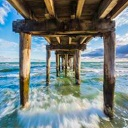
\includegraphics[width=\linewidth, height= 2.5cm]{in2.jpg}
   \caption{Input image}
  \end{subfigure}
  \begin{subfigure}[b]{0.4\linewidth}
    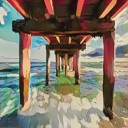
\includegraphics[width=\linewidth, height = 2.5cm]{in2_Hayao.jpg}
    \caption{Output image}
  \end{subfigure}
  \caption{Results of CartoonGAN\cite{Chen2018CartoonGANGA} approach. Here, a real world image (a) is translated a cartoon image (b).}
  \label{fig:carto}
\end{figure}

\section{Proposed Methodology}
The main target of our \textit{cartoon-to-real} is to perform the reverse of CartoonGAN (\textbf{\textit{Cartoon$\rightarrow$Real}}) and we exploit the CycleGAN\cite{zhu2017unpaired} technique for this purpose. The model contains two mapping functions $G:C \rightarrow R$ and $F:R \rightarrow C$ where $C$ denotes cartoon and $R$ denotes the real domain. There are $2$ discriminators ($D_R$, $D_C$) and $2$ generators ($G$, $F$) for the translation process. While performing $C \rightarrow G(C)$, $D_R$ tries to enforce the translation $G(C)$ to domain $R$, and the vice-versa for $D_C$ and $F$. For the regularization, we implement two \textit{cycle consistency losses}\cite{zhu2017unpaired} where authors proposed that the learned mapping functions should be cycle-consistent to avoid direct mapping distribution. The loss is written as -
\begin{multline}
\mathcal{L}_{cyc}(G,F)=\mathds{E}_{c\sim p_{data}(c)}[||F(G(c)) - c||_1] \\
+ \mathds{E}_{r\sim p_{data}(r)}[||G(F(r)) - r||_1]
\end{multline}

Hence, the full objective is -
\begin{multline}
\mathcal{L}(G,F,D_C,D_R)=\mathcal{L}_{GAN}(G,D_R,C,R)\\
\qquad +\mathcal{L}_{GAN}(F,D_C,R,C)\linebreak
+\lambda \mathcal{L}_{cyc}(G, F).
\end{multline}
where $\lambda$ is the weight or relative importance of the two objectives. Therefore, our aim can be described as -
\begin{align}
G^{*},F^{*}&=\text{arg}\,\underset{G,F}{\text{min}}\underset{D_c,D_r}{\text{max}}\mathcal{L}(G,F,D_C,D_R)
\end{align}
\makeatletter
\setlength\@fptop{0pt} 
\setlength\@fpsep{7pt plus 1fil} 
\setlength\@fpbot{0pt}
\makeatother

\begin{figure}
\centering
   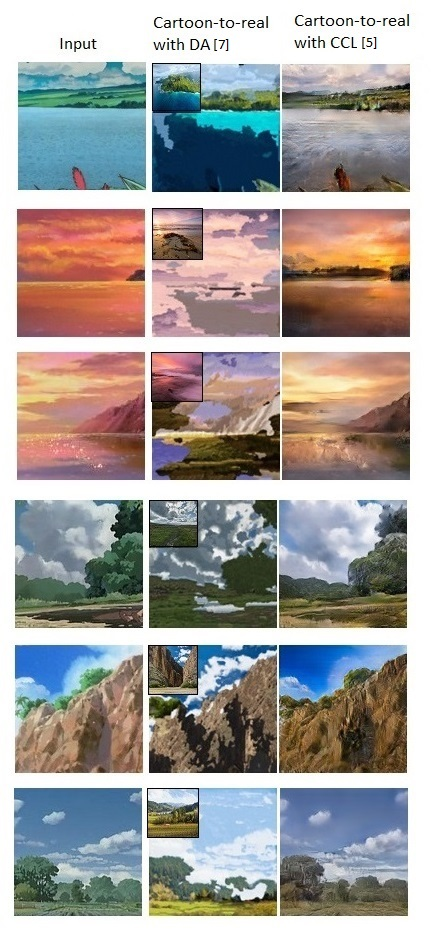
\includegraphics{Comparison-Final2.jpg}  
  
  \caption{Comparison between cartoon to real translation using Deep Analogy (DA) and using cycle consistency loss (CCL). \textit{Left column} shows the input, \textit{middle column} shows the output of using Deep Analogy (with the style image on top corner), and the \textit{right column} presents the results of using cycle consistency loss. It is visible that the cartoon-to-real with cycle consistency loss\cite{zhu2017unpaired} shows the better translation.}

  \label{fig:carto3}
  \end{figure}


\section{Experiment Results}
We developed two unpaired datasets to train our network. For the cartoon domain, we collected almost $3.1$K images scrapped from various movies, e.g. \textit{Pokemon}, \textit{My Neighbour Totoro} and \textit{Kiki's Delivery}. We used \textit{flickr} dataset for the real images' domain. Images are resized to $128 \times 128$ resolution. For implementation we used PyTorch and for hardware we used \texttt{Nvidia GTX $1060$}. We compared our paper with the outputs from another state of the art work called -- \textit{Deep Analogy}\cite{liao2017visual}. Our result along with the outputs from Deep Analogy are presented in Figure~\ref{fig:carto3}. It exhibits that outputs with cycle consistency loss produce more realistic images than that with Deep Analogy.


\section{Conclusion}
In this paper, we performed image translation from cartoons to real world images. We used cycle consistency loss to generate images so that the generate image will not be directly mapped into any distribution of target domain. Our research is yet on progress. However, we observed that our results are not completely satisfactory and our upcoming target is to minimize the limitation. In future, we want to investigate on preserving the content of input image from cartoon domain for better translation.


\bibliographystyle{IEEEtran}
\bibliography{Reference}


% that's all folks
\end{document}


